\documentclass[10pt,pdf,hyperref={unicode}]{beamer}

% \documentclass[aspectratio=43]{beamer}
% \documentclass[aspectratio=1610]{beamer}
% \documentclass[aspectratio=169]{beamer}

\usepackage{lmodern}

% подключаем кириллицу 
\usepackage[T2A]{fontenc}
\usepackage[utf8]{inputenc}

% отключить клавиши навигации
\setbeamertemplate{navigation symbols}{}

% тема оформления
\usetheme{Copenhagen}

% цветовая схема
\usecolortheme{seahorse}

\title{Обучение машинного перевода без параллельных текстов}   
\subtitle{}
\author{Артеменков А.А., Гончаров М.Ю. Ярошенко А.М., Иванов А.В., Мазуров М.Ю., Борисова А.В., Скиднов Е.Д., Строганов Ф.А.} 
\date{\today} 
% \logo{\includegraphics[height=5mm]{images/logo.png}\vspace{-7pt}}

\begin{document}

% титульный слайд
\begin{frame}
	\begin{center}
		\begin{Large}
			
		\end{Large}
	\end{center}
\end{frame}


\begin{frame}
	\frametitle{Список литературы}
	\nocite{lample2017unsupervised} 
	\nocite{graves2005framewise}
	\nocite{kimimproving}
	\nocite{papineni2002bleu}
	\bibliographystyle{unsrt}
	\bibliography{references}
\end{frame}

\begin{frame}
	\frametitle{Постановка задачи}
	
	
	Рассматривается задача построения модели перевода текста без использования параллельных текстов, т.е. пар одинаковых предложений на разных языках.
	
	\textbf{Пример.}
	
	
	\begin{table}[ht]
		\centering
		\begin{tabular}{p{4cm}c| p{4cm}}
			\begin{itemize}
				\item Что это?
				
				\item Вы говорите на украинском языке? 
			\end{itemize}
			& \hfill & 
			\begin{itemize}
				
				\item Що це?
				
				\item Ви говорите українською мовою?
			\end{itemize}
		\end{tabular}
	\end{table}
	
	
	Данная задача возникает при построении моделей перевода для низкоресурсных языков (т.е. языков, для которых данных в открытом доступе немного).
	
	
\end{frame}

\begin{frame}
	\frametitle{Описание эксперимента}
	Для украинско-русской пары:
	\begin{itemize}
		
		\item Непараллельная выборка: мультиязычные статьи из Wikipedia.
		
		\item Параллельный корпус: OpenSubtitles-2018.
		
	\end{itemize}
	
	Для французско-английской пары:
	
	\begin{itemize}
		\item Параллельный корпус: multi30k.
		
		
		\item Метрика измерения качества: BLEU.
		
	\end{itemize} 
	
	Обучение проводилось на обеих выборках, валидация на параллельном корпусе.
	
\end{frame}

\begin{frame}
	\frametitle{Результаты экспериметов}
	
	\begin{figure}[h]
		\centering
		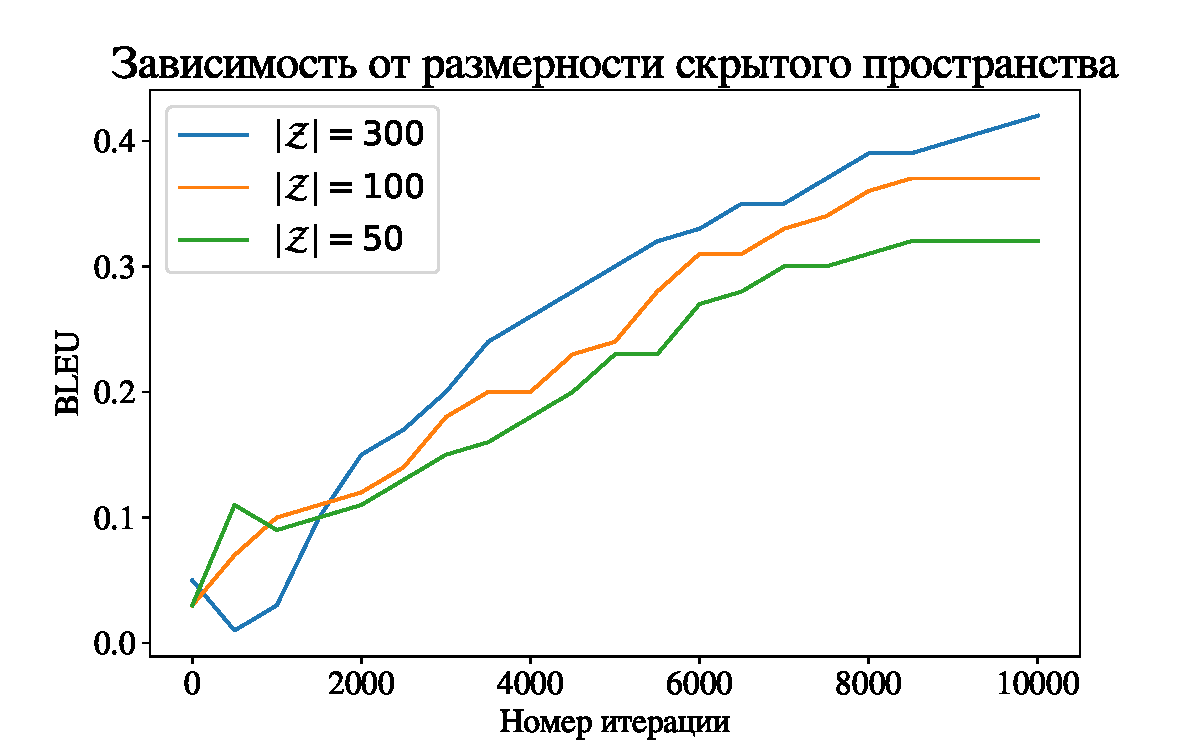
\includegraphics[width=0.7\textwidth]{hidden}
		\caption{Зависимость BLEU от размерности скрытого пространства.}
	\end{figure}
	
\end{frame}

\begin{frame}
	\frametitle{Результаты экспериметов}
	
	\begin{figure}[h]
		\centering
		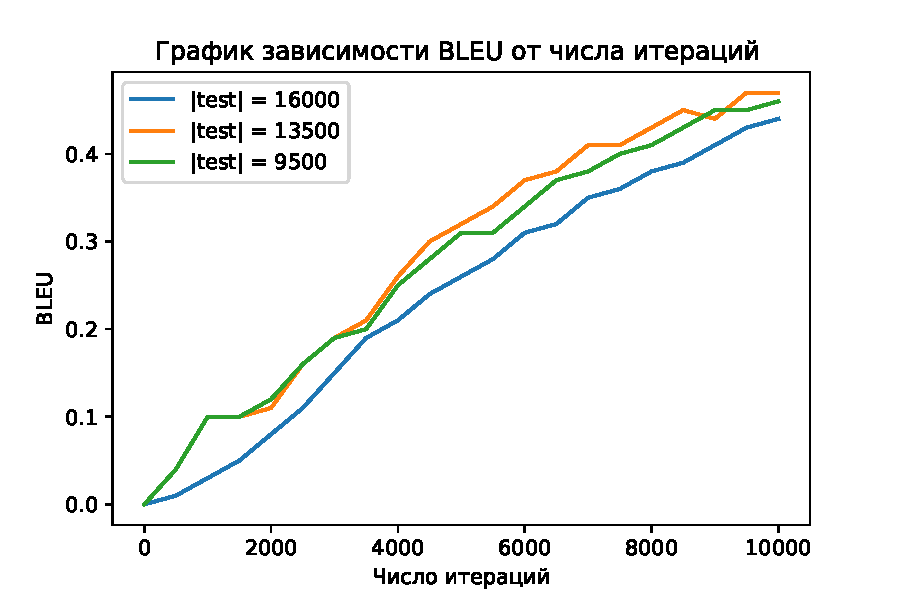
\includegraphics[width=0.7\textwidth]{volume}
		\caption{Зависимость BLEU от размера обучающей выборки.}
	\end{figure}
	
\end{frame}

\begin{frame}
\frametitle{Перевод с русского на украинский язык и обратно} 
\begin{center}
	Проблема: в языках слова могут иметь очень много форм. Из-за этого процесс обучения крайне долгий, вид кривых обучения не меняется кардинально при изменении модели.
	
	\begin{figure}[h]
		\centering
		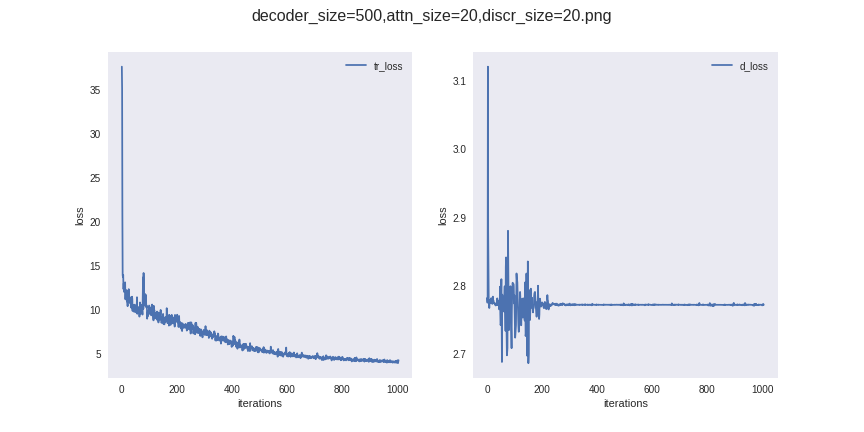
\includegraphics[width=0.9\textwidth]{decoder_size=500,attn_size=20,discr_size=20}
		\caption{Типичный вид кривых обучения на выборке русский-украинский}
	\end{figure}
	
\end{center}
\end{frame}

\begin{frame}
	\frametitle{Некоторое решение - Стемминг!} 
	\begin{center}
		
		\textbf{Стемминг} — процесс нахождения основы слова для заданного исходного слова. Основа слова не обязательно совпадает с морфологическим корнем слова.
		
		\begin{figure}[h]
			\centering
			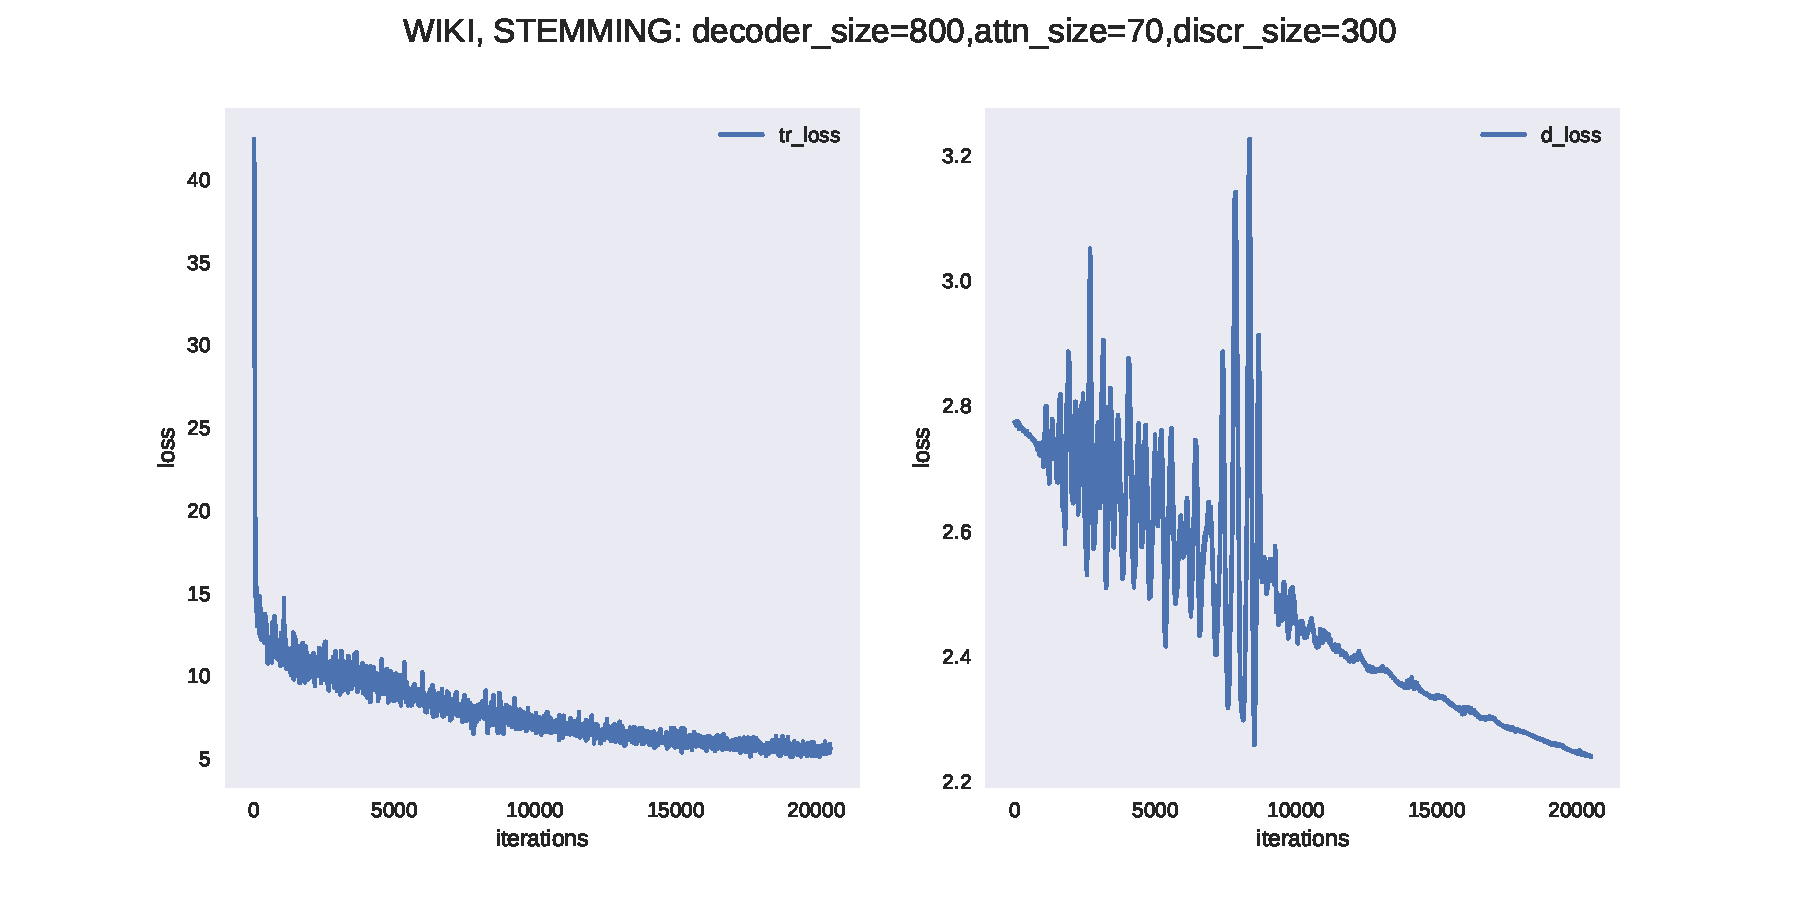
\includegraphics[width=0.9\textwidth]{WIKI,decoder_size=800,attn_size=70,discr_size=300.pdf}
			\caption{Кривые обучения в случае, когда всем словам были удалены последние две буквы}
		\end{figure}
		
	\end{center}
\end{frame}

\begin{frame}
	\frametitle{Некоторое решение - Стемминг!} 
	\begin{center}
	
	\begin{table}[H]
		\caption{\label{tab:canonsummary}Результаты, достигнутые для русско-украинского перевода.}
		\begin{center}
			\begin{tabular}{|c|c|}
				\hline
				Модель(decoder,discriminator,attention) & BLEU после $10^5$ итераций \\
				\hline
				Простая: $100, 100, 50$ & $0.113$ \\
				Промежуточная: $200, 300, 50$ & $0.219$ \\
				Промежуточная: $800, 600, 150$ & $0.222$ \\
				Сложная: $2000, 2000, 150$ & \underline{ $0.293$ } \\
				\hline
				Промежуточная: $800, 300, 70 \; + \; STM$ & $0.413$ \\
				Сложная: $2000, 2000, 150 \; + \; STM$ & $0.427$ \\
				\hline
	
			\end{tabular}
		\end{center}
	\end{table} 
		
	\end{center}
\end{frame}


\end{document}